\documentclass{article}

\usepackage{amsmath,amssymb}
\usepackage{graphicx}
\usepackage{array}
\usepackage[margin=1in]{geometry}
\usepackage{dsfont}

% ===== This makes my \affil cmnd work.
\usepackage[affil-it]{authblk}


% ===== This makes my environments work switching llncs to article.
\newtheorem{theorem}{Theorem}[section]
\newtheorem{lemma}[theorem]{Lemma}
\newtheorem{proposition}[theorem]{Proposition}
\newtheorem{corollary}[theorem]{Corollary}

\newenvironment{proof}[1][Proof]{\begin{trivlist}
\item[\hskip \labelsep {\bfseries #1}]}{\end{trivlist}}
\newenvironment{definition}[1][Definition]{\begin{trivlist}
\item[\hskip \labelsep {\bfseries #1}]}{\end{trivlist}}
\newenvironment{example}[1][Example]{\begin{trivlist}
\item[\hskip \labelsep {\bfseries #1}]}{\end{trivlist}}
\newenvironment{remark}[1][Remark]{\begin{trivlist}
\item[\hskip \labelsep {\bfseries #1}]}{\end{trivlist}}

\newcommand{\qed}{\nobreak \ifvmode \relax \else
      \ifdim\lastskip<1.5em \hskip-\lastskip
      \hskip1.5em plus0em minus0.5em \fi \nobreak
      \vrule height0.75em width0.5em depth0.25em\fi}

% ===== For \algorithm. Is this a decent idea?
\usepackage[lined,boxed,ruled,vlined]{algorithm2e}

% ===== For \mathscr
\usepackage{mathrsfs}
\DeclareSymbolFontAlphabet{\mathrsfs}{rsfs}
\usepackage[mathscr]{eucal}


% ===== For \boldsymbol
\usepackage{amsbsy}

% ===== For \bm (bold math)
\usepackage{bm}

\usepackage{fixltx2e}
\MakeRobust{\overrightarrow}

% ===== For code snippets
\usepackage{courier}

% ==== Misha and Ning's Notation file =====
%% ----------------------------------------------------------------------
%% Definitions, Macros, Etc.
%% ----------------------------------------------------------------------

%% Hyper-linked References
\newcommand{\Sec}[1]{\hyperref[sec:#1]{\S\ref*{sec:#1}}} %section
\newcommand{\Eqn}[1]{\hyperref[eq:#1]{(\ref*{eq:#1})}} %equation
\newcommand{\Fig}[1]{\hyperref[fig:#1]{Figure~\ref*{fig:#1}}} %figure
\newcommand{\Tab}[1]{\hyperref[tab:#1]{Table~\ref*{tab:#1}}} %table
\newcommand{\Thm}[1]{\hyperref[thm:#1]{Theorem~\ref*{thm:#1}}} %theorem
\newcommand{\Lem}[1]{\hyperref[lem:#1]{Lemma~\ref*{lem:#1}}} %lemma
\newcommand{\Prop}[1]{\hyperref[prop:#1]{Property~\ref*{prop:#1}}} %property
\newcommand{\Cor}[1]{\hyperref[cor:#1]{Corollary~\ref*{cor:#1}}} %corollary
\newcommand{\Def}[1]{\hyperref[def:#1]{Definition~\ref*{def:#1}}} %definition
\newcommand{\Alg}[1]{\hyperref[alg:#1]{Algorithm~\ref*{alg:#1}}} %algorithm
\newcommand{\Ex}[1]{\hyperref[ex:#1]{Example~\ref*{ex:#1}}} %example

% Theorem-like constructs
%\newtheorem{example}[theorem]{Example}

% Blackboard fonts 
\newcommand{\Real}{\mathbb{R}}
\newcommand{\Cplx}{\mathbb{C}}
%% Transposes
\newcommand{\Tra}{^{\rm T}} % Transpose
\newcommand{\Cct}{^\dagger} % Complex conjugate transpose

%% Permutation index
\newcommand{\bfpp}{{\bf p}_n}

%% Matrix & Tensor Operations
\newcommand{\Circ}[1]{{\rm circ}\left( #1 \right)}
\newcommand{\Fold}[1]{{\rm fold}\left( #1 \right)}
\newcommand{\Unfold}[1]{{\rm unfold}\left( #1 \right)}
\newcommand{\Twist}[1]{{\rm twist}(\M{#1})}
\newcommand{\Squeeze}[1]{{\rm squeeze}(#1)}
\newcommand{\squeeze}{{\rm squeeze}}
\newcommand{\Mout}{\diamondsuit}
\newcommand{\circu}{ {\rm circ}}
\newcommand{\bcirc}{ {\rm circ}}
\newcommand{\vvec}{ {\rm vec}}

\newcommand{\mc}[1]{\mathcal{#1}}
\newcommand{\mb}[1]{\mathbb{#1}}
\newcommand{\mcr}[1]{\mathrsfs{#1}}

%% Element of complicated object that is surrounded by parens
\newcommand{\PE}[2]{\left( #1 \right)_{#2}}

%% Vector notation
\newcommand{\V}[1]{{\bm{\mathbf{\MakeLowercase{#1}}}}} % vector
\newcommand{\VE}[2]{\MakeLowercase{#1}_{#2}} % vector element

%% Matrix notation
\newcommand{\M}[1]{{\bm{\mathbf{\MakeUppercase{#1}}}}} % matrix
\newcommand{\Mhat}[1]{{\bm{\hat \mathbf{\MakeUppercase{#1}}}}} % matrix
\newcommand{\Mbar}[1]{{\bm{\bar \mathbf{\MakeUppercase{#1}}}}} % matrix
\newcommand{\ME}[2]{\MakeLowercase{#1}_{#2}} % matrix element
\newcommand{\MC}[2]{\V{#1}_{#2}}

%% Tensor notation
\newcommand{\T}[1]{\boldsymbol{\mathscr{\MakeUppercase{#1}}}} %tensor
\newcommand{\TLS}[2]{\M{#1}_{[#2]}} % lateral slice
\newcommand{\TFS}[2]{\M{#1}_{#2}} % frontal slice
\newcommand{\TT}[2]{\V{#1}_{#2}} % tube
\newcommand{\TE}[2]{\MakeLowercase{#1}_{#2}} % tensor element


%% Shortcuts
\newcommand{\TA}{\T{A}}
\newcommand{\TB}{\T{B}}
\newcommand{\TS}{\T{S}}
\newcommand{\TC}{\T{C}}
\newcommand{\TU}{\T{U}}
\newcommand{\TV}{\T{V}}
\newcommand{\TG}{\T{G}}

\newcommand{\Vu}{\V{u}}
\newcommand{\Vv}{\V{v}}
\newcommand{\Vq}{\V{q}}
\newcommand{\Vr}{\V{r}}
\newcommand{\Vp}{\V{p}}
\newcommand{\Vd}{\V{d}}
\newcommand{\Vz}{\V{z}}
\newcommand{\Vb}{\V{b}}
\newcommand{\Vg}{\V{g}}
\newcommand{\Vh}{\V{h}}
\newcommand{\MH}{\M{H}}
\newcommand{\MG}{\M{G}}
\newcommand{\MA}{\M{A}}
\newcommand{\MX}{\M{X}}
\newcommand{\MZ}{\M{Z}}
\newcommand{\MW}{\M{W}}
%\newcommand{\TD}{\T{D}}

\newcommand{\SaS}{{\mathcal S}}

\newcommand{\MGC}{\tilde{\MG}}

\newcommand{\Matlab}{{\sc Matlab}\xspace}
\newcommand{\matlab}{{\sc Matlab}\xspace}
\newcommand{\qtext}[1]{\quad\text{#1}\quad}

\newcommand{\matvec}{{\tt Vec}}
\newcommand{\fld}{{\tt Fold}}

\def \bK{\mathbf{K}}
\def \bF{\mathbf{F}}
\def \bD{\mathbf{D}}
\def \bB{\mathbf{B}}
\def \bA{\mathbf{A}}
\newcommand{\bDelta}{\boldsymbol{\Delta}}

%\newcommand{\bea}{\left[ \begin{array}}
%\newcommand{\eea}{ \end{array} \right]} 

\newcommand{\bftheta}{ {\boldsymbol \theta}}
\newcommand{\bfrho}{ {\boldsymbol \rho}}
\newcommand{\bfeta}{ {\boldsymbol \eta}}
\newcommand{\fft}{ \mbox{\tt fft} }
\newcommand{\ifft}{ \mbox{\tt ifft} }
\newcommand{\blkd}{\mbox{\tt blkdiag}}
\newcommand{\rshpT}{\mbox{\tt reshapeT}}
\newcommand{\F}[1]{\mathcal{F}\{#1\}}
\newcommand{\Fi}[1]{\mathcal{F}^{-1}\{#1\}}
\newcommand{\indep}{\perp\!\!\!\perp}

\usepackage{mathtools}
\DeclarePairedDelimiter{\ceil}{\lceil}{\rceil}
\DeclarePairedDelimiter{\floor}{\lfloor}{\rfloor}
\newcommand{\Var}{\text{Var}}
\newcommand{\E}{\text{E}}
\newcommand{\Cov}{\text{Cov}}



%%%% Dr. K's colored comments. 
\usepackage{color} 
\definecolor{blue}{rgb}{0,0,1}
\definecolor{red}{rgb}{1,0,0}
\definecolor{purple}{rgb}{1,0,1}
\definecolor{gray}{rgb}{0.7,0.7,0.7}
\newcommand\MEK[1]{\textcolor{red}{MEK: #1}}
\newcommand\EMK[1]{\textcolor{purple}{EMK: #1}}
\newcommand\SA[1]{\textcolor{blue}{SA: #1}}
\newcommand\red[1]{\textcolor{red}{#1}}\newcommand\gray[1]{\textcolor{gray}{#1}}
\begin{document}



Eric Kernfeld

Report on Darren Wilkinson's ``Parameter inference for stochastic kinetic models of bacterial gene regulation,'' also referred to as ``the paper'' or ``W10.'' It is a chapter in the proceedings of the ninth Valencia meeting on Bayesian statistics \cite{Bernardo2012}. 

\begin{abstract}
In this paper, Wilkinson attempts to infer reaction rates for biochemical networks in a setting with discrete observations, missing data, and measurement error. He uses vague priors and likelihood-free MCMC methods within a Bayesian model. He runs four main simulations. The first three iterate through successively more difficult and realistic measurement models, and they show the approach can accurately infer three key reaction rates with a useful precision. The fourth studies a naive model, showing it leads to overconfident, incorrect inferences. 

I review some alternative methods in detail and discuss the relative merits of W10's approach. I implement the method in Julia and attempt to reproduce the experiments \EMK{more on this later!}. I assess the method using additional experiments designed to study mixing time, scaling with system size, and prior sensitivity \EMK{more on this later!}. 
\end{abstract}

\tableofcontents
\newpage


\section{Introduction: Parameter Inference for Biological Models}

Modern biology has progressed to the point of creating {\it in silico} models of entire cells. The potential benefit is enormous, because unlike real cells, which must be observed via microscopy or high-throughput methods, a simulated cell can reveal its internal state. The obvious drawback is that simulations do not necessarily correspond to reality either in terms of their mechanisms or in terms of their results. One key limiting factor: even though the structure of biochemical networks is often well known, precise information about how quickly interactions play out has not kept pace. If Protein A promotes transcription of Gene B, and they mix for five minutes, we still need to know whether to expect 10, 100 or 1000 new copies of B's messenger RNA at the end. Wilkinson's paper (W10) confronts a subproblem in this domain.

Chemical reactions are often modeled using ordinary differential equations (ODE's), but Wilkinson's exact subproblem has an extra complication that rules ODE's out: natural stochasticity. W10's model organism\footnote{Held up against the usual meaning in statistics, this use of the word ``model'' is different. Similar to the way that statisticians use models to derive insight about natural phenomena, biologists use particular species to derive broader biological insights. These species are known as model organisms.}
, the bacterium {\it Bacillus subtilis}, varies its behavior so that even if two bacteria begin in similar initial conditions, one may become mobile and the other may not. Here is one explanation, which the underlying physics support and which  Wilkinson's paper subscribes to. Interactions among molecules are themselves random, driven by Brownian motion. If there are only tens or hundreds of molecules, the randomness persists in the system dynamics rather than canceling out. This phenomenon is common, and some natural systems even amplify it in order to produce usefully random behavior \cite{reinker2006parameter}. Wilkinson expresses this in terms of a particular stochastic model, and the main contribution of his paper is a method for inference assuming that model.
 
%In some cases, organisms have mechanisms to reduce this randomness, but in others, as readers fond of rock-paper-scissors might imagine, the random behavior is useful.

\subsection{Poisson process modeling of chemical systems}

For a well-stirred chemical system that maintains thermal equilibrium, Gillespie  \cite{gillespie1992rigorous} derived a model from first principles. The ultimate result is a collection of competing Poisson processes, one for each chemical reaction to be modeled. Suppose there are $x_{i}(t)$ molecules of type $i$ at time $t$, $i\in \{1 ... u\}$. These molecules interact via a set of reactions $\mathcal{R}_{j}$, $j\in \{1 ... v\}$, with $\mathcal{R}_{j}$ consuming $p_{ij}$ particles of type $i$ and producing $q_{ij}$ molecules of type $i$. Let $R_{j}(t)$ denote the number of reactions of type $j$ that happened in $[0,t]$. I'll refer to all these variables collectively using the time-varying vectors $x(t)$ and $R(t)$ along with static matrices $P$ and $Q$. Defining the matrix $S$ to be $Q-P$, the equation $x(t) - x(0) = SR(t)$ shows how the reactions affect the molecule counts. Since the particle counts are integers, the system is not constantly in flux: there will be windows, albeit short ones, where no reactions occur. The exact form of the model is this: over a reaction-free window, $R_{j}(t)$ is a Poisson process with intensity $c_{j}\int_0^t \prod_{i=1}^u {{x_i(t)}\choose{p_{ij}}}$. %Define $h_{i}(c_{i}, x(t)) \equiv c_{i}\int_0^t \prod_{j=1}^u {{x_j(t)}\choose{p_{ij}}}$. 
The $c_{i}$'s are sometimes unknown, and they are the quantities needed for biological models.

\subsection{Inference with complete data and simulation}
Given that every reaction is observed without error, inference is still needed because the system is stochastic. To describe the likelihood, I now describe how to simulate the system.

As with any homogeneous Poisson process, draw an exponential random variable with rate equal to the intensity of the process; that gives the correctly distributed waiting time until the next event. For a collection of independent Poisson processes, use the sum of their intensities as the rate, because in distribution this equals the minimum of the individual wait times (i.e. the first reaction to occur). Choose the type of reaction from a categorical distribution with cell probabilities equal to the normalized intensities. This scheme applies to this setting because even though the process is not homogeneous, it is temporarily homogenous in between reactions. The rates can be recomputed after each new reaction. Popularized by  \cite{gillespie1977}, this is known as the Gillespie algorithm. Pseudocode appears in Algorithm \ref{alg:gillespie}.


\begin{algorithm}[h]
\caption{The Gillespie algorithm \label{alg:gillespie}}
Given:\\
\Indp
A simulation duration $T$\\
$x(0)$, the initial particle counts\\
$S$, a ``stoichiometry matrix'' whose $i,j$ entry says how many molecules of type $i$ appear or vanish in a reaction of type $j$ (net change)\\
$P$, a matrix whose $i,j$ entry says how many molecules of type $i$ enter a rxn of type $j$ (not a net change)\\
$c$, a vector of reaction rates\\
-\\
\Indm
Do this:\\
\Indp
Initialize $x$ to $x(0)$ and $t$ to 0.\\
While true:\\
\Indp
Calculate $\alpha_j = c_j\prod_i {x_i\choose P_{ij}}$\\
Increment $t$ by Exponential($\sum_j \alpha_j$) ($\sum_j \alpha_j$ is the rate parameter)\\
If $t > T$, quit and return $x$.\\
Otherwise, choose an integer $j$ with probability $\frac{\alpha_j}{\sum_j \alpha_j}$.\\
Increment $x$ by adding column $j$ of $S$.\\
\end{algorithm}


Returning to the likelihood, suppose $\nu$ is a vector so that the $i$th reaction has type $\nu_i$ and $t$ is a vector so that the $i$th reaction happens at time $t_i$. The likelihood has a term corresponding to the exponential with the sum of the Poisson intensities. Conditioned on the wait times, the next term consists of the categorical probability given to the actual reaction type observed. That happens for every observed reaction. The normalizing constants of the factors cancel, and at the end of the day, the likelihood is $$L(c|\nu, t) = \prod_{i=1}^n c_{\nu_{i}} \prod_{j=1}^u {{x_{j}(t_{i-1})}\choose{p_{{\nu_{i}}j}}}\exp\left(-c_{\nu_{i}} (t_{i}-t_{i-1}) {{x_j(t_{i})}\choose{p_{{\nu_{i}}j}}}\right).$$

In terms of maximum likelihood inference, this function and its derivatives can be evaluated. In terms of Bayesian inference, it has a conjugate prior (independent Gamma distributions). Computational scale is not an issue: Wilkinson's examples have only 13 molecule types and 18 reactions. The problem arises because of discretely observed data.

\section{Approaching inference without complete data}
\label{sec:intro_em}

In Wilkinson's data, not every reaction is observed. Rather, measurements of molecule counts are taken every five minutes. Many possible sequences of reactions could have resulted in the same observations (infinitely many, counting production-decay or binding-unbinding loops). For each sequence, uncountably many variations exist: consider stretching or shrinking the wait times. Let $\nu$ range over the set of eligible reaction sequences, meaning it matches the observed data. Let $\Omega_{\nu}$ be the set of possible times for reactions in $\nu$. The likelihood becomes 
\begin{equation}\label{eqn_nasty_lik}
L(c|x(0), x(t_1), ... x(T)) =\sum_{\nu}\int_{t\in \Omega_{\nu}} \prod_{i=1}^n c_{\nu_{i}} \prod_{j=1}^u {{x_{j}(t_{i-1})}\choose{p_{{\nu_{i}}j}}}\exp\left(-c_{\nu_{i}} (t_{i}-t_{i-1}) {{x_j(t_{i})}\choose{p_{{\nu_{i}}j}}}\right).
\end{equation}
 %The domain of integration is an n-dimensional simplex in $\mathbb{R}^{n+1}$, and $n$ changes depending on $\nu$. 
The main obstacle here is the summation over reaction sequences. I have not made a serious attempt to evaluate it, and some papers, including W10, claim it is intractable. To further complicate the problem, most reaction sequences are not included in the sum, if we define ``most'' via the measure induced by simulation. In other words, rejection sampling is not a promising approach: most forward simulations, even with correct initial conditions, will not match the data. 

%To my knowledge, this likelihood has not been evaluated.
 Instead, expectation-maximization is a common recourse: alternate between calculating expected complete-data log likelihoods and updating parameters based on that simpler case. Since calculating expected latent reaction times and types is not necessarily possible, as it would be in the case of a time-homogenous process, Horv\'ath and Manini \cite{horvath2008parameter} instead draw samples using the Gillespie method. This produces only trajectories at odds with the observations, which an exact method with infinite computing power could afford to discard. After multiple simulations, they discard all but the trajectory closest to fitting the data, and then they improve the fit of this trajectory by altering some reactions. This makes their method inexact, though they argue the distortion of the likelihood is minimal unless molecule counts are close to zero. Daigle et al. \cite{daigle2012accelerated} take a very similar tactic, using EM with a sampling-based E-step done by rejecting incorrect trajectories. To reduce wasted simulation time, Daigle et al. use a tool they call multi-level splitting, and it bears an eerie resemblence to the sequential sampling method that Wilkinson contributes. Another EM-based method contributed by Bayer et al. \cite{bayer2015stoch_em} confronts the same problem of how to obtain trajectories consistent with data. Their scheme is to simulate forward from one observed time-point and backwards from the next, hoping the two samples meet in the middle. A common theme in this domain is that careful initialization helps reduce the fraction of useless samples. This idea, too, will be mirrored in the Bayesian literature on the topic.

In Wilkinson's work, some molecule counts are zero or close to zero, which renders the approximation in \cite{horvath2008parameter} dubious. Though missing data has not yet been mentioned, at time $t_i$, Wilkinson observes only one molecule out of a system with 13, or in other words one coordinate of the 13-dimensional vector $X(t_i)$. This disqualifies \cite{bayer2015stoch_em} by Bayer et al.'s own admission. The method by Daigle et al., \cite{daigle2012accelerated}, can accomodate partial observations, so it remains competitive, and furthermore it claims to perform better than a different paper co-authored by Wilkinson \cite{Boys2008}. However, \cite{daigle2012accelerated} was published two years after W10. Thus, W10 had no direct competitors when it was published.

%Even if competitive EM-based methods had been available in 2009, 
Wilkinson's papers tend to use Bayesian methods, and they tend to use MCMC for inference. A 2003 paper by Marjoram et al. \cite{Marjoram23122003} opened the way for Metropolis-Hastings samplers that do not require likelihood evaluations. Wilkinson introduces one of these, claims it will not work, and makes, as his paper's main contribution, an adaptation of likelihood-free MCMC (LF-MCMC) for hidden discrete or continuous-time Markov models.

\subsection{Methods similar to Wilkinson's}
\label{MC_backgr}
Wilkinson's adaptation of LF-MCMC is subtle and strange. Because it contains ingredients of several Monte Carlo schemes, the discussion leading up to Wilkinson's algorithm will briefly detour through sequential Monte Carlo and LF-MCMC. Readers familiar with these schemes may wish to skip to the pseudocode in Algorithm \ref{pMCMC} and the attending description. 

On its own, LF-MCMC is just a form of Metropolis-Hastings. To produce samples from a {\it target distribution} $\pi$ over a hidden state $x$ and parameters $\theta$, recall that Metropolis-Hastings says to propose a new sample $x^*, \theta^*$ with distribution $q(x^*, \theta^*|x, \theta)$, then accept the proposal with probability $\min \{1, A\}$ if $A=\frac{q(x, \theta|x^*, \theta^*)}{q(x^*, \theta^*|x, \theta)} \times \frac{\pi(x^*, \theta^*)}{\pi(x, \theta)}$. It will help to keep in mind this ``recipe'' for Metropolis-Hastings, but to motivate and describe LF-MCMC, I move back to the stochastic chemical model.

Suppose we have a set of observations at times $t_i$, $i \in 1...I$, and for each $i$ we label the observations $D_{t_i}$. These might be real-valued scalars measuring brightness from a glowing ``reporter molecule.'' The observations depend on the current hidden state, which is the vector of counts for each molecule type. They may also depend on $\theta$, which aggregates parameters of the measurement error model along with any unknown reaction rates. At time $t_i$, Wilkinson observes only one coordinate of the 13-dimensional vector $x(t_i)$, and it is a noisy observation. On the bright side, the revealed coordinate is fixed and known, and $P(D_{t_{i}}|x(t_i), \theta)$ is assumed to be known and tractable. W09 imposes a prior $P(\theta)$, also tractable. The target distribution for the MCMC is chosen to be the posterior $P(x, \theta|D)$, meaning the term $\frac{P(x^*, \theta^*|D)}{P(x, \theta|D)}$ needs to be computed at each iteration. This term can be rewritten $\frac{P(D|x^*, \theta^*)P(x^*|\theta^*)P(\theta^*)}{P(D|x, \theta)P(x| \theta)P(\theta)}$. The only intractable calculation is $P(x^*|\theta^*)$, which is a special case of Equation \ref{eqn_nasty_lik}. To avoid it, the LF-MCMC comes in.

Marjoram et al.'s LF-MCMC dodges this type of problem not by approximation, but by making the intractable term appear in a second location and cancel the first. In Metropolis-Hastings, each iteration needs the quantity $A=\frac{q(x, \theta|x^*, \theta^*)}{q(x^*, \theta^*|x, \theta)} \times \frac{\pi(x^*, \theta^*)}{\pi(x, \theta)}$. Noticing that the asterisks appear in the numerator for $q$ and the denominator for $\pi$, the inspiration is to build $P(x| \theta)$ into the {\it proposal}. By proposing only $\theta$, then simulating $x$ from the correctly-formed model (here, via the Gillespie algorithm), the entire thing becomes $A=\frac{q(\theta|\theta^*)}{q(\theta^*|\theta)} \frac{P(x|\theta)}{P(x^*|\theta^*)} \times \frac{P(D|x^*, \theta^*)P(x^*|\theta^*)P(\theta^*)}{P(D|x, \theta)P(x| \theta)P(\theta)}$. The intractable terms cancel.

Wilkinson points out that this scheme suffers from the same problem that besets the sampling-based EM: most forward simulations are incongruent with the data. Once the chain gets to taste a single well-placed sample sequence of reactions, it is unlikely to explore parameters and initial conditions other than what produced the winning simulation. The rejection rate is high, and the mixing time is bad. Wilkinson reasonably claims that this problem gets worse with less measurement error or with higher-dimensional observations, and that Marjoram et al.'s method will not work ``out of the box.'' He offers no theory, citations, or experiments to support this claim, except for a clause containing the phrase ``in practice,'' which implies experiments not reported in W10. Wilkinson's work centers around building a sampler with tolerable rejection rates. 

The idea is similar to sequential Monte Carlo (SMC), which uses a sequence of distributions rather than moving directly from proposal to posterior. Most SMC methods resemble importance sampling: propose a collection of independent, identically distributed samples from the wrong distribution. To render the result unbiased, calculate functionals only after appropriately up- or down-weighting each of the samples. 

As is done in this branch of MCMC research, I will begin to refer to each individual sample as a particle. SMC solves a problem in importance sampling where most particle weights are tiny, and just a few particles contribute most of the information. The SMC solution is to introduce several intermediate stages of resampling in which successful particles can multiply and low-weight particles can vanish. Some strategies use perturbations so that the duplicate particles disperse during resampling. If the weights at intermediate stages come from distributions that progress gradually from proposal to target, the effect is a particle cloud slowly migrating into the correct formation. Simple importance sampling would produce a particle cloud whose body all but vanishes and whose wispy edges determine the final estimate. 

Because Wilkinson's scheme involves elements of both SMC and MCMC, it is useful to consider both side by side. In particular, both methods render dependent samples, but for different reasons. In SMC, samples are dependent because many of them have walked randomly away from a common ancestor. MCMC includes the other extreme. If I use an independence proposal, meaning my $q(\theta^*|\theta)$ does not depend on $\theta$, the issue of slow random walks does not arise. Rather, dependence arises because of rejections, in which case $\theta$ must be repeated in order to preserve the correct target density.

\subsection{Inference via Wilkinson's method}
Wilkinson's method indeed lies at this extreme of MCMC: his proposal distribution does not depend on the previous sample. As mentioned in Section \ref{MC_backgr}, dependence arises because of rejects (i.e. repeated samples), and the particle cloud is coaxed into the correct shape because some proposals are rejected more often than others. 

The exact method follows in Algorithm \ref{pMCMC}. As it involves nested loops, pseudocode may be an easier format to read it in, but the essence is this. Draw a large sample from the prior of choice $P(\theta, x(0))$ on the initial state and the parameters. Its empirical distribution will be called the ``current distribution.'' Use the current distribution (or a smoothed version) as a proposal distribution. The first step will convert it to a sample from $P(\theta, x(t_1)|\mathcal{D}_1)$, which indicates two changes. First, the sample comes from a distribution conditioned on one observation, not from the prior, and second, it describes the state at the time of that observation, rather than the initial state. The $i$th step is Metropolis-Hastings, and it results in samples from $P(\theta, x(t_i)|\mathcal{D}_{1}, ...\mathcal{D}_{i})$. It proposes $(x(t_{i-1})^*, \theta^*)$ from the current distribution, then produces $x(t_{i})^*$ via forward simulation using $x(t_{i-1})^*$ as initial the condition and parameters $\theta^*$. It accepts the proposal with probability the lesser of 1 and $A=\min(1, \frac{P(\mathcal{D}_{t_{i}}|x(t_{i})^*, \theta^*)}{P(\mathcal{D}_{t_{i}}|x(t_{i}), \theta)})$. After throwing away the first few states as a burn-in and more as desired to thin out the chain, begin to regard the results as the ``current sample'' and move to the next iteration. Repeat that until no data remains.

To be clear, instead of running MCMC just once, this method runs another five million steps through the sampler for every time point in the dataset. It is not as outrageous as it sounds; many competitors scale linearly in both the forward simulation cost and the length of the Markov chain. %for a sampler that runs only once, the chain will not mix without a sophisticated proposal, and constructing a usable proposal is often linear in the size of the data anyway.
For example, the approximate likelihood used in every MCMC step in \cite{golightly2011bayesian} is linear in the time-series' length, and the differential equations giving the approximate likelihood inside the MCMC loop in \cite{milner2013moment} and \cite{zechner2012moment} are analogous to forward simulations.

\begin{algorithm}[h]
\caption{ \label{pMCMC} Wilkinson's sequence of MCMC Samplers}
Given a hidden continuous-time Markov process $\{x_t\}_{t=0}^T$ with: \\
\Indp \Indp
Unknown parameters $\theta$\\
Known initial state $x_0$\\
Data points $\mathcal{D}_{t_{i}}$ at times $t_{i}$, $i \in \{1, ... I\}$ \\
A simple, tractable error model $P(\mathcal{D}_{t_{i}}|x(t_{i}), \theta)$\\
A simulator for paths of $x$ given $\theta$ the process\\
A big array $B_0$ (Wilkinson uses length 1,000,000) of samples from a prior on $\theta, x_0$\\
Empty arrays $B_{i}$ of the same length\\
$\phantom{0}$\\
\Indm \Indm
For each time point (for $i \in \{1, ... I\}$), fill $B_{i}$ with samples from this Metropolis-Hastings scheme:\\
\Indp\Indp
Initialize $(\theta, x(t_{i}))$ \\
Until $B_{i}$ is full: \\
\Indp\Indp
Draw $(\theta^*, x(t_{i-1})^*)$ from $B_{i-1}$ or a kernel density estimate (KDE) from its contents (note $t_0\equiv0$)\\
Using $(\theta^*, x(t_{i-1})^*)$, simulate up to $x(t_{i})^*$, the state at time $t_{i}$ \\
Set $A=\min(1, \frac{P(\mathcal{D}_{t_{i}}|x(t_{i})^*, \theta^*)}{P(\mathcal{D}_{t_{i}}|x(t_{i}), \theta)})$\\
With probability $A$, overwrite $(\theta, x(t_{i}))$ with $(\theta^*, x(t_{i})^*)$\\
If the number of times through this loop exceeds 1000 (for the burn-in) and equals one modulo five (for the thinning), add $(\theta, x(t_{i}))$ to $B_{i}$\\
\Indm \Indm
\end{algorithm}
\pagebreak
Why is the target as claimed? To be precise, this would be done by mathematical induction, but I show only a proof that stage $i$ is correct given stage $i-1$ is correct. From the Metropolis-Hastings recipe, the acceptance probability is either $1$ or the proposal ratio times the posterior ratio. For step $i$, the proposal ratio $\times$ posterior ratio can be expanded as follows. The posterior ratio is written as a ratio of filtering probabilities $P(\mathcal{D}_{t_{i}}, x(t_{1:i}), \theta|\mathcal{D}_{t_{i:i-1}})$.
\begin{align*}
\underbrace{\frac{P(x(t_{i})^*| x(t_{1:i-1})^*,\theta^*\gray{, \mathcal{D}_{t_{1:i-1}}})}{P(x(t_{i})| x(t_{1:i-1}), \theta \gray{, \mathcal{D}_{t_{1:i-1}}})}}_{\text{forward simulation}}
%
&\overbrace{\frac{P(x(t_{1:i-1})^*,\theta^*| \mathcal{D}_{t_{1:i-1}})}{P(x(t_{1:i-1}), \theta| \mathcal{D}_{t_{1:i-1}})}}^{\text{induction hypothesis}}
%
\times \\
%
&\underbrace{\frac{P(x(t_{i})| x(t_{1:i-1}), \theta \gray{, \mathcal{D}_{t_{1:i-1}}})}{P(x(t_{i})^*| x(t_{1:i-1})^*,\theta^*\gray{, \mathcal{D}_{t_{1:i-1}}})}}_{\text{...then look here...}}
%
\overbrace{\frac{ P(x(t_{1:i-1}), \theta| \mathcal{D}_{t_{1:i-1}})}{ P( x(t_{1:i-1})^*,\theta^*| \mathcal{D}_{t_{1:i-1}})} }^{\text{For a joint PDF, start here...}}
%  
\underbrace{\frac{P(\mathcal{D}_{t_{i}}|x(t_{i}), \theta\gray{, \mathcal{D}_{t_{1:i-1}}})}{P(\mathcal{D}_{t_{i}}|x(t_{i})^*, \theta^*\gray{, \mathcal{D}_{t_{1:i-1}}})}}_{\text{...and finally, look here.}}
%
.\end{align*} 
Most of this cancels, which shows how the brief expression in Algorithm \ref{pMCMC} arises. Notice the gray terms: the hidden Markov model structure lets us include or omit them at will. This is key: otherwise the proposal, which is not conditioned on the data directly, would not cancel the intractable likelihood term, which conditions on the data. As a side note, using a KDE affects this ratio, because the densities $\frac{P(x(t_{i-1})^*,\theta^*| \mathcal{D}_{t_{i-1}})}{P(x(t_{i-1}), \theta| \mathcal{D}_{t_{i-1}})}$ in the proposal get convolved with the kernel but their counterparts in the target do not.% Second, as written the algorithm and the proof do not address the joint distribution of the state over all times. By recording the history of the state for each particle, the algorithm can sample from $P(x(t_{0:I})|\mathcal{D}_{t_{0:I}})$; in the proof, replace $t_{i-1}$ with $t_{0:i-1}$ to see this. 

\section{Pros, Cons and Experiments}


\subsection{Replication and sample impoverishment}

Wilkinson runs four main experiments, all of them roughly identical. In each of them, he uses a 13-molecule, 18-reaction system. He creates simulated data from the Poisson process model, generating 24 observations at 300-second intervals and adding Gaussian noise with a standard deviation of 10 molecules. He treats the noise distribution as known, along with all but three reaction rates. His experiments are biologically motivated: a different molecule is observed each in each experiment, and the results show which molecules contain enough information to pin down the parameters. In the fourth experiment, the form of the model is mis-specified, and he shows that this leads to strong and incorrect posteriors.

Figure \ref{fig:SigD_trial_may27} is representative of the results of the experiments done with properly specified models. It shows a contour plot of the posterior density over two of three unknown log parameters. The correlation in the posterior appears because the parameters represent binding and unbinding of the same pair of molecules. Chemical systems exist in dynamic equilibrium; in other words, near-constant amounts of a substance reflect equal rates of gain and loss rather than underlying stasis. Given a dynamic equilibrium with some molecules bound together and others free, uncertainty remains about how dynamic the equilibrium is.

\begin{figure}[h!]
\begin{center}
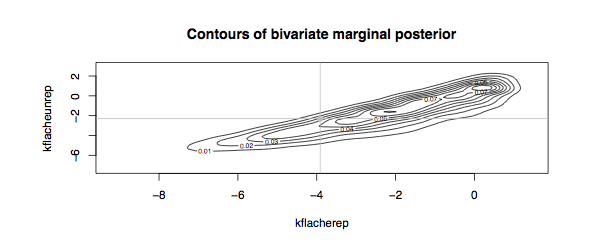
\includegraphics[height=2in,width=4in]{wilkinson_fig3_biv.png}
\caption{ \label{fig:SigD_trial_may27} Bivariate marginal of the posterior from Wilkinson's figure 3. Axes show log reaction rates for binding and unbinding rates of two molecules. True rates appear as intersecting gray lines.}
\end{center}

\end{figure}


Because these experiments were similar to one another and biologically motivated, I plan to reproduce only one before moving on to experiments that answer statistical questions. These other experiments are motivated in the next section.


\subsubsection{Sample impoverishment}
Sequential Monte Carlo suffers from a problem termed sample impoverishment, which means that eventually most samples are duplicates of a common ancestor and few unique values remain. Plots of results even with 1,000,000 samples seem to display this issue. To document this criticism fully, Figure \ref{fig:SigD_trial_may27} shows the posterior distribution over two unknown rates from a replicate of one of W10's experiments. In the synthetic data, twenty-four observations occurred at intervals of 300 seconds, with a noise sd of 10.0. There were 1,000,000 particles, with true rates and log-uniform priors matching Wilkinson's. The acceptance rate in the first round was 2 percent, but it ranged between 25 and 95 percent thereafter. Though the posterior is scattered around the true value, the plot indicates few unique particles persisting to the final round. 

%: \log(kSigDprod) ∼ Unif(\log\{0.01\}, \log\{100\}),\log(kflacherep) ∼ Unif(\log\{0.0002\}, \log\{2\}),\log(kflacheunrep) ∼ Unif(\log\{0.001\}, log\{10\})

\begin{figure}[h!]
\begin{center}
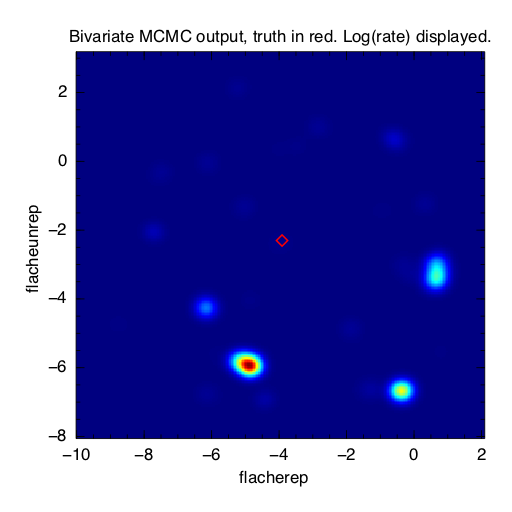
\includegraphics[height=4in,width=4in]{SigD_trial_small_bw_may27.png}
\caption{Bivariate marginal of the posterior from an attempted replication of Wilkinson's figure 3. Axes show log reaction rates for binding and unbinding rates of two molecules. True rates appear as a red diamond.}
\end{center}
\label{fig:SigD_trial_may27}
\end{figure}

This warrants a brief analysis. Wilkinson records the first of every five samples for use in the next stage's proposal. Ten rejections in a row thus guarantees a repeat. Recording the empirical rejection rates from the trial in the figure and taking each to the tenth power gives convervative estimates of the rate of 10-rejections-in-a-row, as if the trials were independent. This seems charitable: rejections could be correlated, since any small string of rejections signals a desirable starting point and perhaps more rejections to come. Converting these to rates of at-least-one-acceptance-after-10-rounds, we get proportions $p_i$ such that $N$ unique particles before stage $i$ will result in about $Np_i$ unique particles after stage $i$. Multiplying the stages together, the result is about 0.0003. So, being charitable, I would expect the final sample to have about 3 unique values for every 10,000 in the prior sample.

In fact, this treats the method too kindly for another reason: I would expect some more repeats to arise because the proposal distribution will begin to contain repeats. When proposed, these might be more likely to be accepted, as they were already selected to be probable based on earlier data. 

Wilkinson, with lead author Andrew Golightly, criticizes W10's sample impoverishment problem in a later paper \cite{golightly2011bayesian}. 

\paragraph{Solutions to sample impoverishment}
Interestingly, the highest rejection rates are concentrated in the first couple of rounds, when moving between $P(\theta)$ and $P(\theta|\mathcal{D}_{t_1})$ and $P(\theta|\mathcal{D}_{t_1}, \mathcal{D}_{t_2})$. This suggests a simple adaptation: spend more effort in the first round, perhaps by thinning more aggressively. \EMK{Haven't tried this extension yet.}

Another solution to this problem is to sample from a KDE of the previous distribution, rather than just resampling. %Wilkinson mentions using a KDE instead of straight resampling, but he does not explain how important it is, and he does not mention any of the literature (for example \cite{particle_filter_tutorial}) that helps explain why and how to carry out a KDE in this setting.  Using a KDE renders the method no longer exact, but according to \cite{particle_filter_tutorial}, it works better than no KDE. %The paper \cite{particle_filter_tutorial} also gives a rule for bandwidth selection. 
Unfortunately, using a KDE in log-space with a normal kernel, sd of 0.05, yields the density in Figure \ref{fig:SigD_trial_may27}: a small cloud, centered tightly in the wrong place, with a smattering of other misplaced modes. This is not a genuine improvement over a point-mass posterior estimate. 

Using a wider kernel would ideally allow the particle cloud to diffuse, then evaporate from less likely areas and persist wherever the mode(s) should be. Indeed, a trial run with a bandwidth of 0.5 and 1,000,000 particles assigns more substantial density near the true value. There is still cause for worry, though: W10 gives higher rates than the truth for both reactions, which makes sense because lower-than-expected binding could mask lower-than-expected unbinding. This replication makes mistakes in opposite directions for the two coordinates. Furthermore, W10 shows a thin, diagonal posterior: the method consistently opted for matched binding and unbinding rates. Even though W10's results are based on unpublished, simulated data and the replication is based on different data, the results should share a basic property like posterior correlation.

\begin{figure}[h!]
\begin{center}
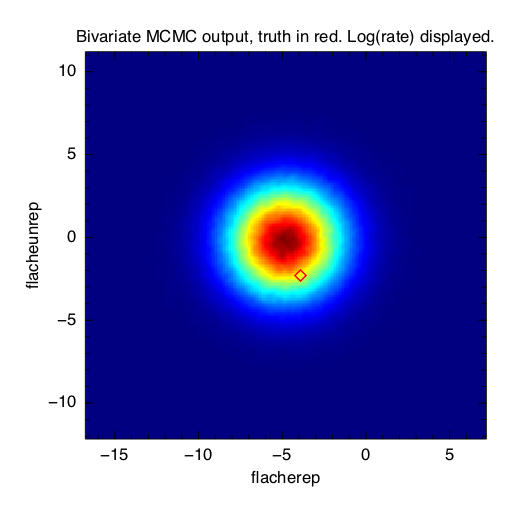
\includegraphics[height=4in,width=4in]{SigD_trial_large_bw_may_29.png}
\caption{Bivariate marginal of the posterior from a large-bandwidth attempt at replicating Wilkinson's figure 3. Axes show log reaction rates for binding and unbinding rates of two molecules. True rates appear as a red diamond. \label{fig:SigD_trial_may29}}
\end{center}

\end{figure}

\paragraph{A more basic experiment}
At this point, it made sense to ask whether the method could generate sensible posterior estimates in a simple system. I encoded a system with only one molecule, using a constant, unknown immigration rate and a constant, unknown decay rate. Figure \ref{fig:simple_test} shows the results. After the first data point, a sensible stripe appears. Then the particle cloud begins to degenerate into an immobile sphere.

\begin{figure}[h!]
\begin{center}
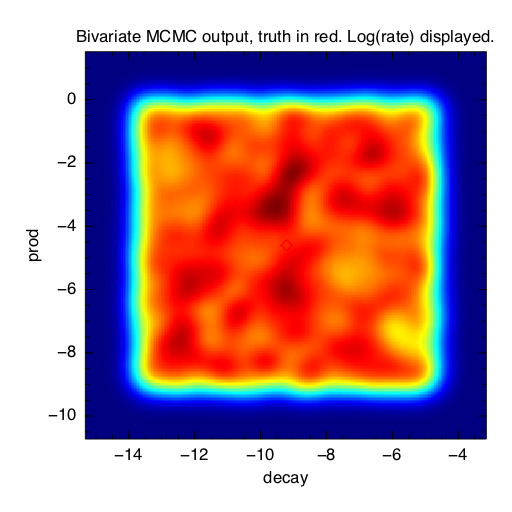
\includegraphics[height=1in,width=1in]{simple_million_stagewise_plots/dist0_contour_decay_prod.png}
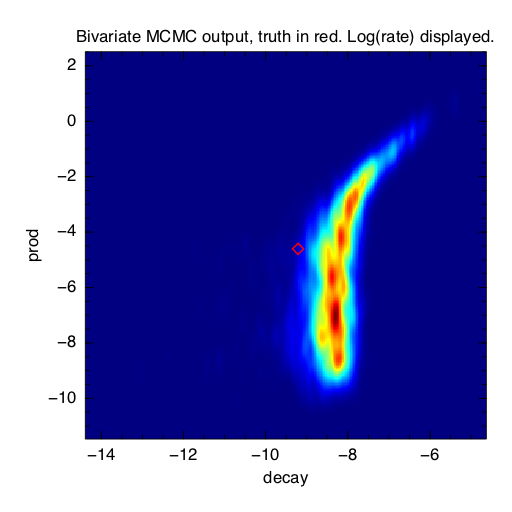
\includegraphics[height=1in,width=1in]{simple_million_stagewise_plots/dist1_contour_decay_prod.png}
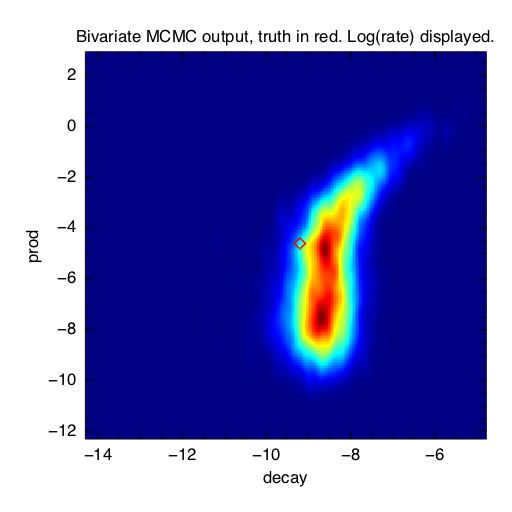
\includegraphics[height=1in,width=1in]{simple_million_stagewise_plots/dist2_contour_decay_prod.png}
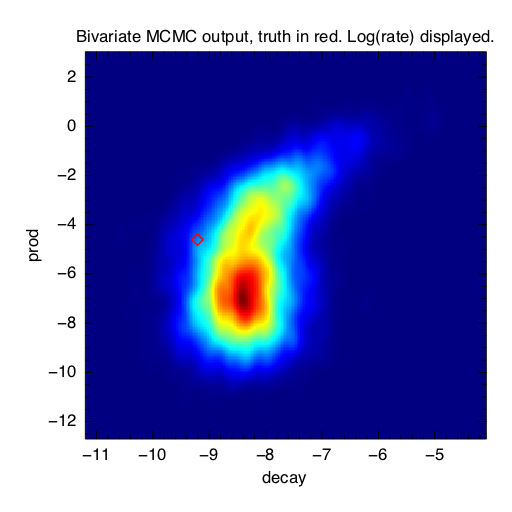
\includegraphics[height=1in,width=1in]{simple_million_stagewise_plots/dist3_contour_decay_prod.png}
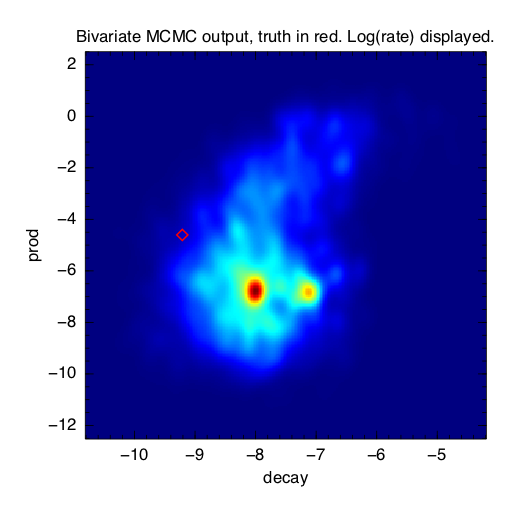
\includegraphics[height=1in,width=1in]{simple_million_stagewise_plots/dist4_contour_decay_prod.png}
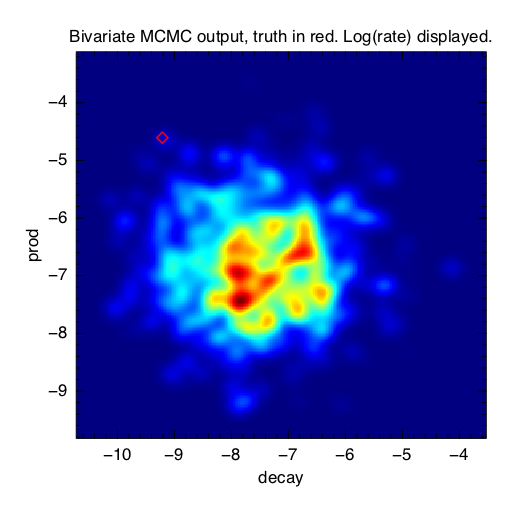
\includegraphics[height=1in,width=1in]{simple_million_stagewise_plots/dist23_contour_decay_prod.png}
\caption{Bivariate marginals of the distribution of production (vertical) and decay (horizontal) log rates in a simple system. From left to right, distributions condition on zero data points, one, two, three, four, and 24. \label{fig:simple_test}}
\end{center}

\end{figure}

\paragraph{Returning to bandwidth selection}
Bandwidth selection is important, and there is no theory to guide it here, but the state of the art is to take an out-of-the-box rule and divide the resulting bandwidth by ten \cite{wilk_email}. \EMK{I will write about this experiment when it finishes.}

\subsection{Pros and Cons}
\subsubsection{Computing time}
Wilkinson's example lies at a scale tailored to custom experiments with far fewer molecules and reactions than the whole-cell efforts cited earlier. The entire system describes only 13 molecules and 18 reactions. The experiments use a synthetic time-series with only 24 measurements. Attempting to replicate these results using Wilkinson's priors, my Julia-language implementation of the method takes about two days to run. As opposed to Matlab or R, Julia offers fast performance, including loops, to mimic that of a statically typed language, and my implementation has been optimized using the Julia \texttt{@profile} macro. Wilkinson also notes computation time as an area for improvement, particularly when processing data from entire batches of cells undergoing the same experiment.

A notable weakness of this algorithm is that it cannot be parallelized at any stage. Looking at the outside loop, each time a data point is added, the whole chain must be run before adding another data point, because the proposals depend on the previous stage having finished. Within a single chain, each calculation depends on the state of the chain, which depends on the previous calculation. Within each iteration, the forward simulation consumes the bulk of the power, but this too is a Markov process requiring serial computation. One sensible modification would be to run many chains at each stage, burning each of them in separately. Wilkinson does not report running multiple chains.

\subsubsection{Modeling error}
All of Wilkinson's experiments use synthetic data, generated from the correct model. Having neglected all but the most important chemicals, Wilkinson bears the burden of showing that modeling error in this reduced model is not too great. The method can perform no better than the model it is given, and this is doubly true because even if better models exist, the method is not computationally viable for bigger systems. Wilkinson stresses that much more information about his example network is available than is used, but offers no citations to show that his reduction works well or that, in general, models can isolate a dozen molecules out of a complicated biochemical soup and still perform well.

If model error is possible, that raises another question: how much extra effort towards exact inference is warranted? W10 is meant to study systems for which a diffusion approximation does not serve, but would some other approximation be worthwhile?

\subsubsection{Mixing time}
Wilkinson discards 1000 samples as a burn-in at every stage of the sampler. Is this sufficient? He offers experiments showing scenarios where the method does or doesn't give good results, but he never addresses this concern about whether it is working properly, not even via citation or theoretical mixing time analysis. Meanwhile, other authors using MCMC describe discarding far more of their samples as a burn-in, between 10 and 50 percent \cite{gupta2014comparison,zechner2014scalable}. A simple experiment to address this concern: run the sampler twice using W10's settings (1,000,000 particles, a thin of 5, and a burnin of 1,000). Both runs should yield similar results if the inference is to be trusted. \EMK{I am running this experiment.}

\subsubsection{Prior Selection (cons)}
In experiments, Wilkinson's priors cover four orders of magnitude, but they are centered (on a log scale) exactly over the true parameters. Are the results robust to choices of prior that merely cover the true values? \EMK{I will experiment with this once I finish the replication.}

\subsubsection{Prior Selection (pros)}
Unlike some competitors, W10's priors need not be dictated by convenience.

\subsubsection{Flexibility}
Wilkinson's approach is wonderfully adaptable. On the surface, Marjoram et al.'s LF-MCMC makes no HMM assumption and so is more flexible, but Wilkinson claims convincingly that LF-MCMC does not mix properly in this setting. The technique of constructing intermediate distributions by adding one datum at a time would generalize to any hidden Markov model, and coupled with the likelihood-free approach, this allows tremendous flexibility for indirect observation of stochastic and/or nonlinear systems. Adaptation for different types of observation (for example, a fluorescent protein instead of the protein of interest) is simple. Wilkinson points out that posteriors could be fed straight back into the algorithm as priors to analyze a second dataset, and this approach allows for analysis of different models that share parameters. The main aspect limiting flexibility was already mentioned: computing cost.



\section{Discussion and alternative methods}
This area seems to have progressed rapidly starting around 2006: Reinker et al write in \cite{reinker2006parameter} that they are not aware of methods that can cope with measurement error in systems with few molecules. In 2008, Boys \textit{et al.} write ``...we believe this is
the first systematic attempt to conduct rigorous `exact' inference for partially and discretely observed stochastic kinetic models'' \cite{Boys2008}. Now, in mid-2015, many strategies exist. In fact, there is too much to describe it all unless I am to turn this project into a review paper. I attempt to digest and organize a sort of a snowball sample of this literature, centering around the citations within W10. Some papers, based on EM, are described in Section \ref{sec:intro_em}. Others include methods of moments, variational inference, and myriad adaptations of MCMC. My main concerns in assessing these models are tolerance for missing data and scaling.

\subsection{Moment closure}
Some schemes, such as \cite{milner2013moment}, \cite{kugler2012moment}, and \cite{zechner2012moment}, match moments to choose parameters. The core of these methods is an analytically-derived differential equation system that changes with the parameters. The system is typically infinite in size: only an infinite number of moments can completely encode the distributions that arise from the model. To facilitate a solution, higher moments are set to zero; this gives rise to the term ``moment closure'' that describes the methods. For each set of candidate parameters, the system is solved numerically. In \cite{milner2013moment}, the end result is a setup where quickly-solvable ODE's for mean and covariance give a Gaussian to approximate the true density, and \cite{milner2013moment} embeds this inside of a Bayesian random-walk MCMC scheme. To distinguish this MCMC from LF-MCMC, it does evaluate an approximation to the likelihood: that is exactly what the moments are used for. MCMC also appears in \cite{zechner2012moment}. There, MCMC functions as a search algorithm to maximize an approximate posterior, which is evaluated as the prior times a moment-based normal approximation to the likelihood. Thus, these schemes require solving multidimensional ODE systems inside of MCMC samplers. The project  \cite{kugler2012moment} uses a penalty function involving higher moments, rather than a moment-matched approximate density. Despite being less interpretable in terms of probability theory, the results in a fast procedure that allows for partial observations, as well as some assessment of uncertainty through repeated runs. For more information on different uses of moment closure, \cite{Milner201199} cites many applied projects using it. W10 precedes all of this work. 

\subsection{Variational inference}
Mean-field variational inference approximates a posterior distribution by finding a nearby joint distribution whose coordinates are independent. For Markov jump processes, one effort at mean field variational inference \cite{opper2008variational} scales well for large systems. This work precedes W10 by a year and has some intriguing properties. It is one of few inference methods in this subfield that requires no sampling or stochastic search, and it allows for fairly flexible priors on hidden states. W10's hidden state priors arise implicitly from his parameter priors and initial state priors, meaning that in the hidden state, they treat only uncertainty due to intrinsic randomness (aleatory uncertainty), but in the parameters they treat uncertainty due to incomplete knowledge (epistemic uncertainty). Thus, (\cite{opper2008variational}) offers a way to bring in outside information about specific transitions that W10 lacks.

To estimate parameters, \cite{opper2008variational} would need to be extended, perhaps as part of a variational EM algorithm. As written, the variational approximation is for the latent states, not parameters. Even variational EM does not give estimates of parameter uncertainty, so this work is not a viable alternative to W10 for scientific parameter estimation. For even more evidence that \cite{opper2008variational} cannot handle parameter estimation properly, the method gives intervals with close-to-nominal coverage except when attempting projection, and authors attribute this failure to untreated parameter uncertainty. 

\subsection{Maximum \textit{\textbf{ a posteriori}} inference}
James Rawlings' group has developed sampling algorithms that produce a semianalytical posterior distribution or likelihood over $\theta$, which they then optimize using derivative-free methods similar to simulated annealing \cite{gupta2014comparison,srivastava_rawlings2014stoch_opt}.   This work came after W10 by five years. They use an ingenious importance sampling scheme: if $q$ is the importance distribution, the idea starts as
\begin{align*}
P(\theta|D) &= \int_x P(\theta|x)P(x|D) dx\\
&\approx \sum_x P(\theta|x)\frac{P(x|D)}{q(x)} dx\\
&\approx \frac{1}{P(D)}\sum_x P(\theta|x)\frac{P(D|x)P(x)}{q(x)} dx.
\end{align*}
$P(D|x)$ is tractable. So is $P(\theta|x)$ if a conjugate gamma prior is used. They deal with $\frac{1}{P(D)}$ by normalizing the importance weights, and $P(x)$ they evaluate in closed form as $\frac{P(x|\theta)P(\theta)}{P(\theta|x)}$, which is a ratio of gamma distribution normalizing constants. 

This requires use of gamma priors, which is a restriction: the posterior is a mixture of many gammas, so it cannot be recycled as the prior when processing a new dataset. Also, domain experts 
often use log-normal or log-uniform priors, as does W10, and both sources regard prior choice as important. However, the scheme is exact, and well-designed $q$ can make it more efficient than MCMC-based schemes. If the prior choice issue could be resolved, this alternative might be well suited to Wilkinson's problem. 

\subsection{Bayesian inference via MCMC}
As noted, there is too much to literature on parameter estimation to cover all of it in this project. Paradoxically, focusing on ``only'' the ones using MCMC seems to make the problem worse. Bearing in mind that this review is incomplete, a good jumping-off point might be \cite{golightly2011bayesian}, because (like W10) it uses multiple common techniques. One numerical trick in particular bears mention: sometimes, likelihood terms appearing in proposal ratios can be replaced with noisy but unbiased estimates 
%
\footnote{Surprisingly, this works even with biased estimates, as long as the bias does not depend on the parameters being sampled.}
%
, and the target distribution will still be correct (details appear in \cite{andrieu2010particle}). This lets \cite{golightly2011bayesian} embed an SMC estimate of the intractable discrete-data likelihood inside of a random-walk MCMC scheme, retaining exactness. The price: noisy likelihood approximations at each step make for a slower mixing chain overall; the noisier, the slower. Furthermore, the SMC inside the main loop requires forward simulations from the Gillespie algorithm. Though SMC can be run in parallel, communication between processors at every new proposal makes this impractical. Displeased with the computational cost of SMC incurred at each iteration, \cite{golightly2011bayesian} employs another trick: they approximate the process using a continuous-state diffusion process satisfying a certain SDE. The SDE itself is intractable, so they use an Euler approximation to draw samples. 

The paper \cite{owen2014scalable} is similar to \cite{golightly2011bayesian}, with both using the acceptance-ratio approximation from \cite{andrieu2010particle}. In \cite{owen2014scalable}, though, multiple chains are run in parallel. To reduce burn-in costs, which scale with the number of processors used, \cite{owen2014scalable} initializes each chain from an inexact importance-sampling-like procedure known as Approximate Bayesian Computation (ABC) that can be run in parallel. Other permutations and combinations of MCMC, SMC, SDE/ODE approximation, and ABC appear in the literature. For more on ABC, the paper \cite{owen2014ABC_LF-MCMCcomparison} compares it against exact methods. Other papers using SDE approximations or related techniques include \cite{golightly2005bayesian}, \cite{Boys2008} and \cite{fearnhead2014inference}.

For most methods, endpoint-conditioned simulation is the primary issue in this problem; it affects LF-MCMC, sampling-based EM schemes, and (indirectly, via the SMC estimate variance) the schemes in \cite{golightly2011bayesian,owen2014scalable}. The paper \cite{golightly2014smc_b_subtilis} would have been another good jumping-off point, as it explores several proposal-generating options and offers a rich set of references. The paper \cite{amrein2012rate} is also noteworthy for detailing a tidy, though approximate, solution. The set of eligible reaction totals given the change in chemical counts is phrased as a lattice, a vector-space-like set containing only integers. A matrix spanning it is obtained, and it suffices to multiply a random vector of integers into that matrix. This work in \cite{amrein2012rate} is sophisticated enough to deal with partial measurements at a given time point, and it anticipates and deals with the potential criticism (e.g. \cite{golightly2011bayesian}) that separate block updates to parameters and latent state can lead to low acceptance rates.

The paper \cite{zechner2014scalable} is similar to W10, using MCMC updates inside a sequential Monte Carlo scheme. This work is a step up from the rest in terms of model complexity, treating batches of cells with some shared parameters and some parameters that vary by cell. The mathematical machinery involves extra tools to marginalize over between-cell variability and block updates in places where Wilkinson doesn't need them. 

\subsection{Conclusions}
For a statistician working in 2009, W10 was a big step forward. Statistically, it is a feat: exact inference using discrete data, measured with error, to infer parameters of an arbitrary stochastic nonlinear system, with reasonable quantification of uncertainty, and all without a single likelihood evaluation. Unfortunately, the restrictions imposed to reach this combination of properties leave little room to adapt the method for parallel processing or in ways that would improve mixing. For a mathematical biologist shopping for parameter inference algorithms, I recommend newer algorithms like \cite{owen2014scalable}%, \cite{gupta2014comparison}
 or \cite{zechner2014scalable}. These scale better than W10, taking advantage of the flexibility offered by the method of moments or the particle marginal Metropolis-Hastings algorithm \cite{andrieu2010particle}.

%\begin{algorithm}[h]
%\caption{ Sequential ABC\label{algo:ABC} }
%Given: \\
%\Indp \Indp
%Unknown parameters $\theta$\\
%Data points $\mathcal{D}_{t_{i}}$ at times $t_{i}$, $i \in \{1, ... I\}$ \\
%A symmetric kernel $K(\cdot)$ and tuning parameters $\epsilon_i$\\
%A simulator for paths of $x$ given $\theta$ the process\\
%A length-$N$ array $B_0$ of samples from a prior on $\theta, x_0$\\
%Empty arrays $B_{i}$ of the same length, $N$\\
%An array $\Omega_{i}$ of length $N$\\
%$\phantom{0}$\\
%\Indm \Indm
%For each time point (for $i \in \{1, ... I\}$), fill $B_{i}$ with samples from this scheme:\\
%\Indp\Indp
%Initialize $(\theta, x(t_{i}))$ \\
%Until $B_{i}$ is full: \\
%\Indp\Indp
%Draw $(\theta^*, x(t_{i-1})^*)$ from index $j$ of $B_{i-1}$ with probability $\omega_j$
%Using $(\theta^*, x(t_{i-1})^*)$, simulate up to $x(t_{i})^*$, the state at time $t_{i}$ \\
%If $\rho()$, overwrite $(\theta, x(t_{i}))$ with $(\theta^*, x(t_{i})^*)$\\
%If the number of times through this loop exceeds 1000 (for the burn-in) and equals one modulo five (for the thinning), add $(\theta, x(t_{i}))$ to $B_{i}$\\
%\Indm \Indm
%\end{algorithm}



%\begin{figure}[h!]
%\begin{center}
%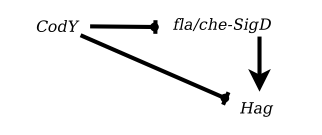
\includegraphics[scale=0.5]{wilkinson_reg_network.png}
%\caption{Regulatory relationships. $Hag$ is the gene for $flagellin$, while $SigD$ encodes $\sigma^D$.}
%\end{center}
%\label{fig:}
%\end{figure}


\begin{align*}
\end{align*}
\begin{align*}
\end{align*}
\begin{align*}
\end{align*}
\begin{align*}
\end{align*}

%\texttt{code snippet}
%
%\begin{algorithm}[h]
%\caption{ }
%Do things\\
%Loop:\\
%\Indp
% Do this again and again\\
%\end{algorithm}

%\begin{figure}[h!]
%\begin{center}
%\includegraphics[height=4in,width=6in]{filename.pdf}
%\caption{}
%\end{center}
%\label{fig:}
%\end{figure}

%$\left[
%\begin{tabular}{ >{$}c<{$} >{$}c<{$}}
% 1 & -\phi_1\\
% -\phi_1 & 1
%\end{tabular} 
%\right]$

%==== Bib files and style =======
\bibliographystyle{splncs}
\bibliography{prelim_biblio}
\end{document}
